\section{dg::Image Class Reference}
\label{classdg_1_1Image}\index{dg::Image@{dg::Image}}
{\tt \#include $<$Image.h$>$}

Collaboration diagram for dg::Image:\begin{figure}[H]
\begin{center}
\leavevmode
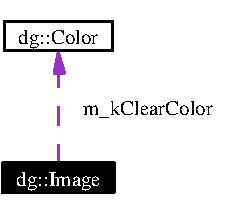
\includegraphics[width=75pt]{classdg_1_1Image__coll__graph}
\end{center}
\end{figure}
\subsection*{Public Methods}
\begin{CompactItemize}
\item 
{\bf Image} ({\bf UInt} ui\-Width=0, {\bf UInt} ui\-Height=0, {\bf UInt} ui\-Channels=0, const {\bf Color} \&rk\-Clear\-Color={\bf Color::GRAY})
\item 
{\bf $\sim$Image} ()
\item 
const {\bf Real} $\ast$ {\bf operator[$\,$]} ({\bf UInt} ui\-Index) const
\item 
{\bf Real} $\ast$ {\bf operator[$\,$]} ({\bf UInt} ui\-Index)
\item 
const {\bf Real} $\ast$ {\bf operator()} ({\bf UInt} ui\-X, {\bf UInt} ui\-Y, {\bf UInt} ui\-C) const
\item 
{\bf Real} $\ast$ {\bf operator()} ({\bf UInt} ui\-X, {\bf UInt} ui\-Y, {\bf UInt} ui\-C)
\item 
{\bf Color} {\bf operator()} ({\bf UInt} ui\-X, {\bf UInt} ui\-Y) const
\item 
{\bf UInt} {\bf index} ({\bf UInt} ui\-X, {\bf UInt} ui\-Y, {\bf UInt} ui\-C) const
\item 
{\bf UInt} {\bf width} () const
\item 
{\bf UInt} {\bf height} () const
\item 
{\bf UInt} {\bf channels} () const
\item 
{\bf UInt} {\bf get\-Width} () const
\item 
{\bf UInt} {\bf get\-Height} () const
\item 
{\bf UInt} {\bf get\-Channels} () const
\item 
const {\bf Real} $\ast$ {\bf pixels} () const
\item 
{\bf Real} $\ast$ {\bf pixels} ()
\item 
const {\bf Real} $\ast$ {\bf get\-Pixels} () const
\item 
{\bf Real} $\ast$ {\bf get\-Pixels} ()
\item 
{\bf Color} {\bf get\-Color} ({\bf UInt} ui\-X, {\bf UInt} ui\-Y) const
\item 
void {\bf set\-Color} ({\bf UInt} ui\-X, {\bf UInt} ui\-Y, const {\bf Color} \&rk\-Color)
\item 
{\bf Color} {\bf get\-Clear\-Color} () const
\item 
void {\bf set\-Clear\-Color} (const {\bf Color} \&rk\-Color)
\item 
void {\bf resize} ({\bf UInt} ui\-Width, {\bf UInt} ui\-Height, {\bf UInt} ui\-Channels)
\item 
void {\bf blur} ()
\end{CompactItemize}


\subsection{Constructor \& Destructor Documentation}
\index{dg::Image@{dg::Image}!Image@{Image}}
\index{Image@{Image}!dg::Image@{dg::Image}}
\subsubsection{\setlength{\rightskip}{0pt plus 5cm}Image::Image ({\bf UInt} {\em ui\-Width} = 0, {\bf UInt} {\em ui\-Height} = 0, {\bf UInt} {\em ui\-Channels} = 0, const {\bf Color} \& {\em rk\-Clear\-Color} = {\bf Color::GRAY})}\label{classdg_1_1Image_a0}




Definition at line 9 of file Image.cpp.

References dg::Real, and dg::UInt.\index{dg::Image@{dg::Image}!~Image@{$\sim$Image}}
\index{~Image@{$\sim$Image}!dg::Image@{dg::Image}}
\subsubsection{\setlength{\rightskip}{0pt plus 5cm}Image::$\sim$Image ()}\label{classdg_1_1Image_a1}




Definition at line 29 of file Image.cpp.

\subsection{Member Function Documentation}
\index{dg::Image@{dg::Image}!blur@{blur}}
\index{blur@{blur}!dg::Image@{dg::Image}}
\subsubsection{\setlength{\rightskip}{0pt plus 5cm}void Image::blur ()}\label{classdg_1_1Image_a23}




Definition at line 58 of file Image.cpp.

References dg::Real, and dg::UInt.

Referenced by dg::Ray\-Tracer::render().\index{dg::Image@{dg::Image}!channels@{channels}}
\index{channels@{channels}!dg::Image@{dg::Image}}
\subsubsection{\setlength{\rightskip}{0pt plus 5cm}{\bf UInt} dg::Image::channels ()\hspace{0.3cm}{\tt  [inline]}}\label{classdg_1_1Image_a10}




Definition at line 142 of file Image.h.\index{dg::Image@{dg::Image}!getChannels@{getChannels}}
\index{getChannels@{getChannels}!dg::Image@{dg::Image}}
\subsubsection{\setlength{\rightskip}{0pt plus 5cm}{\bf UInt} dg::Image::get\-Channels ()\hspace{0.3cm}{\tt  [inline]}}\label{classdg_1_1Image_a13}




Definition at line 167 of file Image.h.\index{dg::Image@{dg::Image}!getClearColor@{getClearColor}}
\index{getClearColor@{getClearColor}!dg::Image@{dg::Image}}
\subsubsection{\setlength{\rightskip}{0pt plus 5cm}{\bf Color} dg::Image::get\-Clear\-Color ()\hspace{0.3cm}{\tt  [inline]}}\label{classdg_1_1Image_a20}




Definition at line 205 of file Image.h.\index{dg::Image@{dg::Image}!getColor@{getColor}}
\index{getColor@{getColor}!dg::Image@{dg::Image}}
\subsubsection{\setlength{\rightskip}{0pt plus 5cm}{\bf Color} dg::Image::get\-Color ({\bf UInt} {\em ui\-X}, {\bf UInt} {\em ui\-Y}) const\hspace{0.3cm}{\tt  [inline]}}\label{classdg_1_1Image_a18}




Definition at line 182 of file Image.h.\index{dg::Image@{dg::Image}!getHeight@{getHeight}}
\index{getHeight@{getHeight}!dg::Image@{dg::Image}}
\subsubsection{\setlength{\rightskip}{0pt plus 5cm}{\bf UInt} dg::Image::get\-Height ()\hspace{0.3cm}{\tt  [inline]}}\label{classdg_1_1Image_a12}




Definition at line 162 of file Image.h.\index{dg::Image@{dg::Image}!getPixels@{getPixels}}
\index{getPixels@{getPixels}!dg::Image@{dg::Image}}
\subsubsection{\setlength{\rightskip}{0pt plus 5cm}{\bf Real} $\ast$ dg::Image::get\-Pixels ()\hspace{0.3cm}{\tt  [inline]}}\label{classdg_1_1Image_a17}




Definition at line 177 of file Image.h.\index{dg::Image@{dg::Image}!getPixels@{getPixels}}
\index{getPixels@{getPixels}!dg::Image@{dg::Image}}
\subsubsection{\setlength{\rightskip}{0pt plus 5cm}const {\bf Real} $\ast$ dg::Image::get\-Pixels ()\hspace{0.3cm}{\tt  [inline]}}\label{classdg_1_1Image_a16}




Definition at line 172 of file Image.h.\index{dg::Image@{dg::Image}!getWidth@{getWidth}}
\index{getWidth@{getWidth}!dg::Image@{dg::Image}}
\subsubsection{\setlength{\rightskip}{0pt plus 5cm}{\bf UInt} dg::Image::get\-Width ()\hspace{0.3cm}{\tt  [inline]}}\label{classdg_1_1Image_a11}




Definition at line 157 of file Image.h.\index{dg::Image@{dg::Image}!height@{height}}
\index{height@{height}!dg::Image@{dg::Image}}
\subsubsection{\setlength{\rightskip}{0pt plus 5cm}{\bf UInt} dg::Image::height ()\hspace{0.3cm}{\tt  [inline]}}\label{classdg_1_1Image_a9}




Definition at line 137 of file Image.h.

Referenced by dg::Visualizer::draw\-Hypertexture(), dg::Visualizer::draw\-Raytraced(), dg::Ray\-Tracer::render(), dg::Hypertexture::render(), and dg::Camera::setup().\index{dg::Image@{dg::Image}!index@{index}}
\index{index@{index}!dg::Image@{dg::Image}}
\subsubsection{\setlength{\rightskip}{0pt plus 5cm}{\bf UInt} dg::Image::index ({\bf UInt} {\em ui\-X}, {\bf UInt} {\em ui\-Y}, {\bf UInt} {\em ui\-C}) const\hspace{0.3cm}{\tt  [inline]}}\label{classdg_1_1Image_a7}




Definition at line 127 of file Image.h.\index{dg::Image@{dg::Image}!operator()@{operator()}}
\index{operator()@{operator()}!dg::Image@{dg::Image}}
\subsubsection{\setlength{\rightskip}{0pt plus 5cm}{\bf Color} dg::Image::operator() ({\bf UInt} {\em ui\-X}, {\bf UInt} {\em ui\-Y}) const\hspace{0.3cm}{\tt  [inline]}}\label{classdg_1_1Image_a6}




Definition at line 114 of file Image.h.\index{dg::Image@{dg::Image}!operator()@{operator()}}
\index{operator()@{operator()}!dg::Image@{dg::Image}}
\subsubsection{\setlength{\rightskip}{0pt plus 5cm}{\bf Real} $\ast$ dg::Image::operator() ({\bf UInt} {\em ui\-X}, {\bf UInt} {\em ui\-Y}, {\bf UInt} {\em ui\-C})\hspace{0.3cm}{\tt  [inline]}}\label{classdg_1_1Image_a5}




Definition at line 105 of file Image.h.\index{dg::Image@{dg::Image}!operator()@{operator()}}
\index{operator()@{operator()}!dg::Image@{dg::Image}}
\subsubsection{\setlength{\rightskip}{0pt plus 5cm}const {\bf Real} $\ast$ dg::Image::operator() ({\bf UInt} {\em ui\-X}, {\bf UInt} {\em ui\-Y}, {\bf UInt} {\em ui\-C}) const\hspace{0.3cm}{\tt  [inline]}}\label{classdg_1_1Image_a4}




Definition at line 96 of file Image.h.\index{dg::Image@{dg::Image}!operator[]@{operator[]}}
\index{operator[]@{operator[]}!dg::Image@{dg::Image}}
\subsubsection{\setlength{\rightskip}{0pt plus 5cm}{\bf Real} $\ast$ dg::Image::operator[$\,$] ({\bf UInt} {\em ui\-Index})\hspace{0.3cm}{\tt  [inline]}}\label{classdg_1_1Image_a3}




Definition at line 88 of file Image.h.\index{dg::Image@{dg::Image}!operator[]@{operator[]}}
\index{operator[]@{operator[]}!dg::Image@{dg::Image}}
\subsubsection{\setlength{\rightskip}{0pt plus 5cm}const {\bf Real} $\ast$ dg::Image::operator[$\,$] ({\bf UInt} {\em ui\-Index}) const\hspace{0.3cm}{\tt  [inline]}}\label{classdg_1_1Image_a2}




Definition at line 80 of file Image.h.\index{dg::Image@{dg::Image}!pixels@{pixels}}
\index{pixels@{pixels}!dg::Image@{dg::Image}}
\subsubsection{\setlength{\rightskip}{0pt plus 5cm}{\bf Real} $\ast$ dg::Image::pixels ()\hspace{0.3cm}{\tt  [inline]}}\label{classdg_1_1Image_a15}




Definition at line 152 of file Image.h.\index{dg::Image@{dg::Image}!pixels@{pixels}}
\index{pixels@{pixels}!dg::Image@{dg::Image}}
\subsubsection{\setlength{\rightskip}{0pt plus 5cm}const {\bf Real} $\ast$ dg::Image::pixels ()\hspace{0.3cm}{\tt  [inline]}}\label{classdg_1_1Image_a14}




Definition at line 147 of file Image.h.

Referenced by dg::Visualizer::draw\-Hypertexture(), and dg::Visualizer::draw\-Raytraced().\index{dg::Image@{dg::Image}!resize@{resize}}
\index{resize@{resize}!dg::Image@{dg::Image}}
\subsubsection{\setlength{\rightskip}{0pt plus 5cm}void Image::resize ({\bf UInt} {\em ui\-Width}, {\bf UInt} {\em ui\-Height}, {\bf UInt} {\em ui\-Channels})}\label{classdg_1_1Image_a22}




Definition at line 35 of file Image.cpp.

References dg::Real, and dg::UInt.

Referenced by dg::Visualizer::setup\-Hypertexture(), and dg::Visualizer::setup\-Ray\-Tracer().\index{dg::Image@{dg::Image}!setClearColor@{setClearColor}}
\index{setClearColor@{setClearColor}!dg::Image@{dg::Image}}
\subsubsection{\setlength{\rightskip}{0pt plus 5cm}void dg::Image::set\-Clear\-Color (const {\bf Color} \& {\em rk\-Color})\hspace{0.3cm}{\tt  [inline]}}\label{classdg_1_1Image_a21}




Definition at line 210 of file Image.h.

Referenced by dg::Visualizer::setup\-Ray\-Tracer().\index{dg::Image@{dg::Image}!setColor@{setColor}}
\index{setColor@{setColor}!dg::Image@{dg::Image}}
\subsubsection{\setlength{\rightskip}{0pt plus 5cm}void dg::Image::set\-Color ({\bf UInt} {\em ui\-X}, {\bf UInt} {\em ui\-Y}, const {\bf Color} \& {\em rk\-Color})\hspace{0.3cm}{\tt  [inline]}}\label{classdg_1_1Image_a19}




Definition at line 195 of file Image.h.

Referenced by dg::Ray\-Tracer::render(), and dg::Hypertexture::render().\index{dg::Image@{dg::Image}!width@{width}}
\index{width@{width}!dg::Image@{dg::Image}}
\subsubsection{\setlength{\rightskip}{0pt plus 5cm}{\bf UInt} dg::Image::width ()\hspace{0.3cm}{\tt  [inline]}}\label{classdg_1_1Image_a8}




Definition at line 132 of file Image.h.

Referenced by dg::Visualizer::draw\-Hypertexture(), dg::Visualizer::draw\-Raytraced(), dg::Ray\-Tracer::render(), dg::Hypertexture::render(), and dg::Camera::setup().

The documentation for this class was generated from the following files:\begin{CompactItemize}
\item 
{\bf Image.h}\item 
{\bf Image.cpp}\end{CompactItemize}
